%%%%%%%%%%%%%%%%%%%%%%%%%%%%%%%%%%%%%%%%%%%%%%%%%%%%%%%%%%%%%%%%%%%%%%%%%%%%%%%%%%
\begin{frame}[fragile]\frametitle{}
\begin{center}
{\Large Chatbot Platforms}
\end{center}
\end{frame}

%%%%%%%%%%%%%%%%%%%%%%%%%%%%%%%%%%%%%%%%%%%%%%%%%%%%%%%%%%%
 \begin{frame}[fragile]\frametitle{Bot Building Platforms}
\begin{itemize}
\item Set of tools and architecture
\item To help you design unique conversation scenarios, define corresponding actions and analyze interactions.
\item Understand Natural language (NLU—Natural language understanding), 
\item Process the conversation text and extracts information (NLP—Natural Language Processing) and \item Respond to the user preserving the context of the conversation (NLG—Natural Language Generation).
\end{itemize}

{\tiny (Ref: Chatbots 101 - Architecture \& Terminologies -  Bhavani Ravi)}

\end{frame}

%%%%%%%%%%%%%%%%%%%%%%%%%%%%%%%%%%%%%%%%%%%%%%%%%%%%%%%%%%%
\begin{frame}[fragile]\frametitle{Typical Chatbot Platform}


\begin{center}
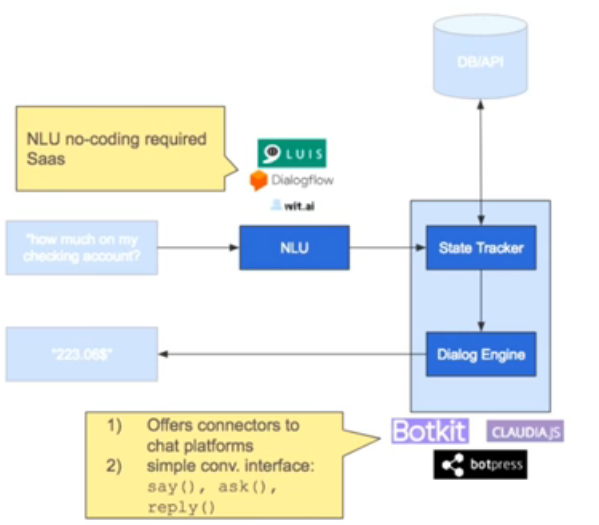
\includegraphics[width=0.6\linewidth]{rasa25}
\end{center}

NLU is over net and Dialog management is still if-and-else.

{\tiny (Ref: The talk would be about Rasa, an open-source chatbots platform - Nathan Zylbersztejn)}

\end{frame}


%%%%%%%%%%%%%%%%%%%%%%%%%%%%%%%%%%%%%%%%%%%%%%%%%%%%%%%%%%%
 \begin{frame}[fragile]\frametitle{Conversation Platforms}
 Established players
\begin{itemize}
\item Google DialogFlow : https://dialogflow.com
\item Facebook Wit.ai : https://www.wit.ai
\item IBM Watson Assistant : https://www.ibm.com/cloud/watson-assistant/
\item Microsoft LUIS : https://www.luis.ai/
\item Amazon Lex : https://aws.amazon.com/lex
\item RASA : https://www.rasa.com/
\end{itemize}

\begin{center}
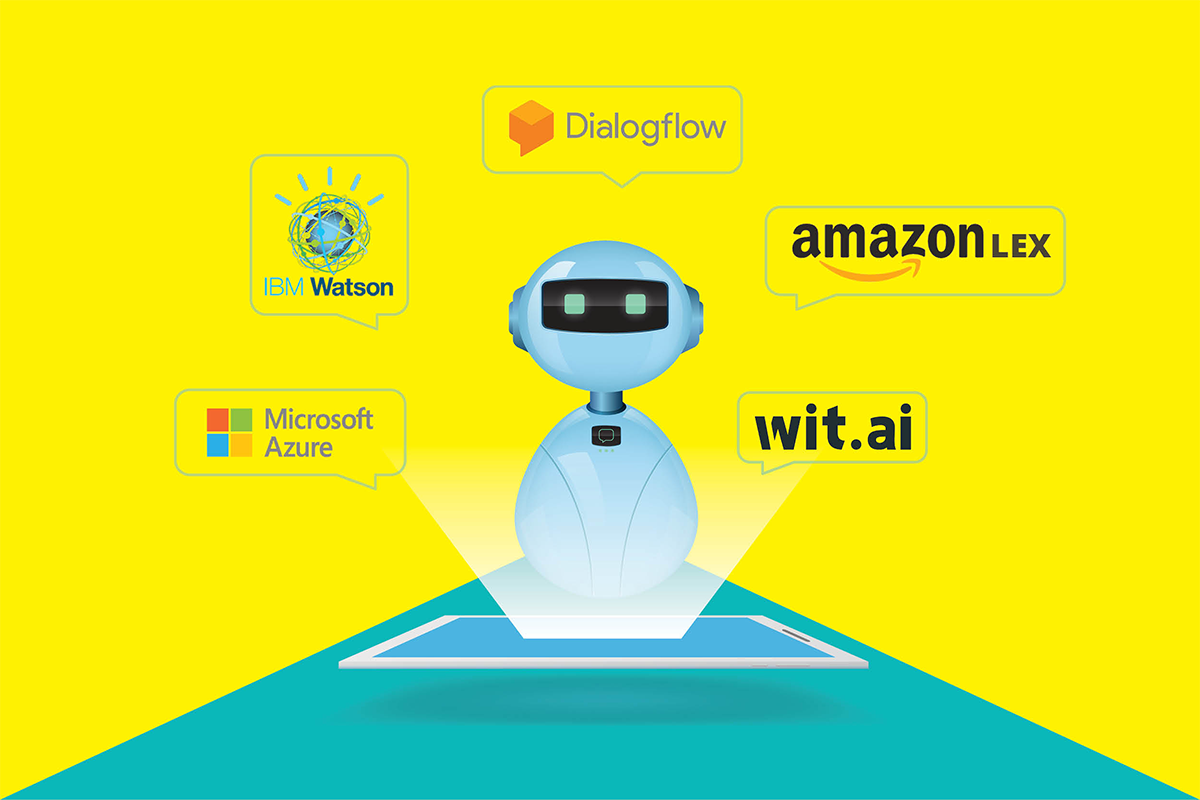
\includegraphics[width=0.5\linewidth]{chatbot56}

\tiny{(Ref : Dialogflow vs Lex vs Watson vs Wit vs Azure Bot | Which Chatbot Service Platform To Use?)}
\end{center}

\end{frame}

%%%%%%%%%%%%%%%%%%%%%%%%%%%%%%%%%%%%%%%%%%%%%%%%%%%%%%%%%%%
 \begin{frame}[fragile]\frametitle{Google Dialogflow}
\begin{itemize}
\item Previous known as API.ai
\item Completely closed-source product with APIs and web interface.
\item Voice and text-based conversational interface
\item Easy to even non-techies to create basic bots. 
\end{itemize}

\begin{center}
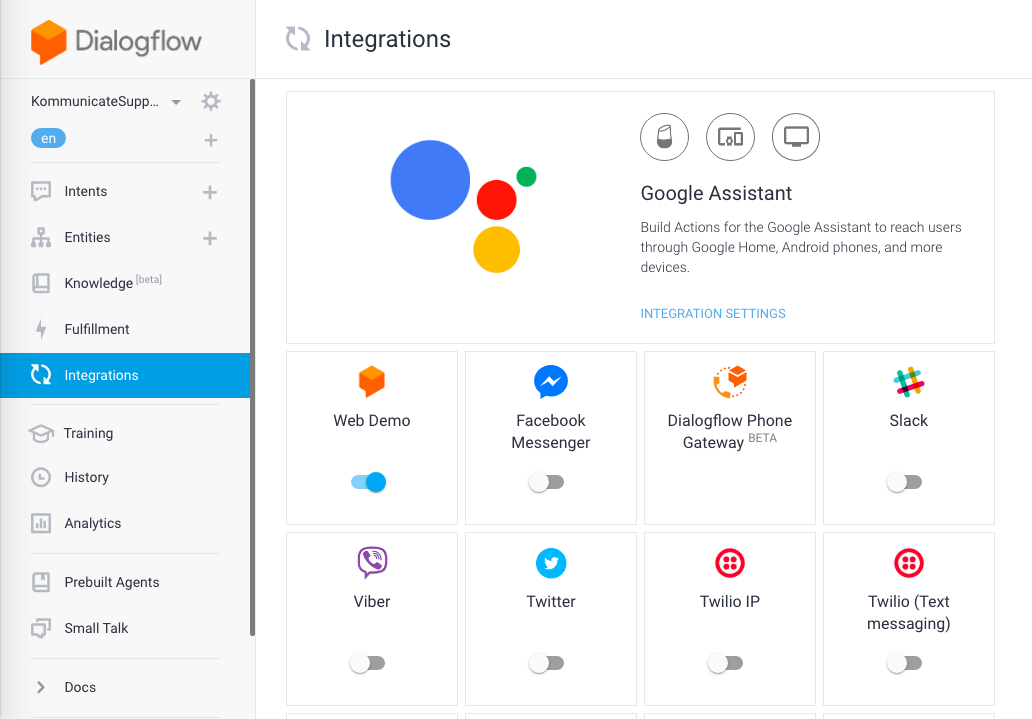
\includegraphics[width=0.6\linewidth]{chatbot57}

\tiny{(Ref : Dialogflow vs Lex vs Watson vs Wit vs Azure Bot | Which Chatbot Service Platform To Use?)}
\end{center}
\end{frame}

%%%%%%%%%%%%%%%%%%%%%%%%%%%%%%%%%%%%%%%%%%%%%%%%%%%%%%%%%%%
 \begin{frame}[fragile]\frametitle{Amazon Lex}
\begin{itemize}
\item Same deep learning technologies as Alexa
\item Voice and text-based conversational interface
\item Provides a web interface to create and launch bots.
\end{itemize}

\begin{center}
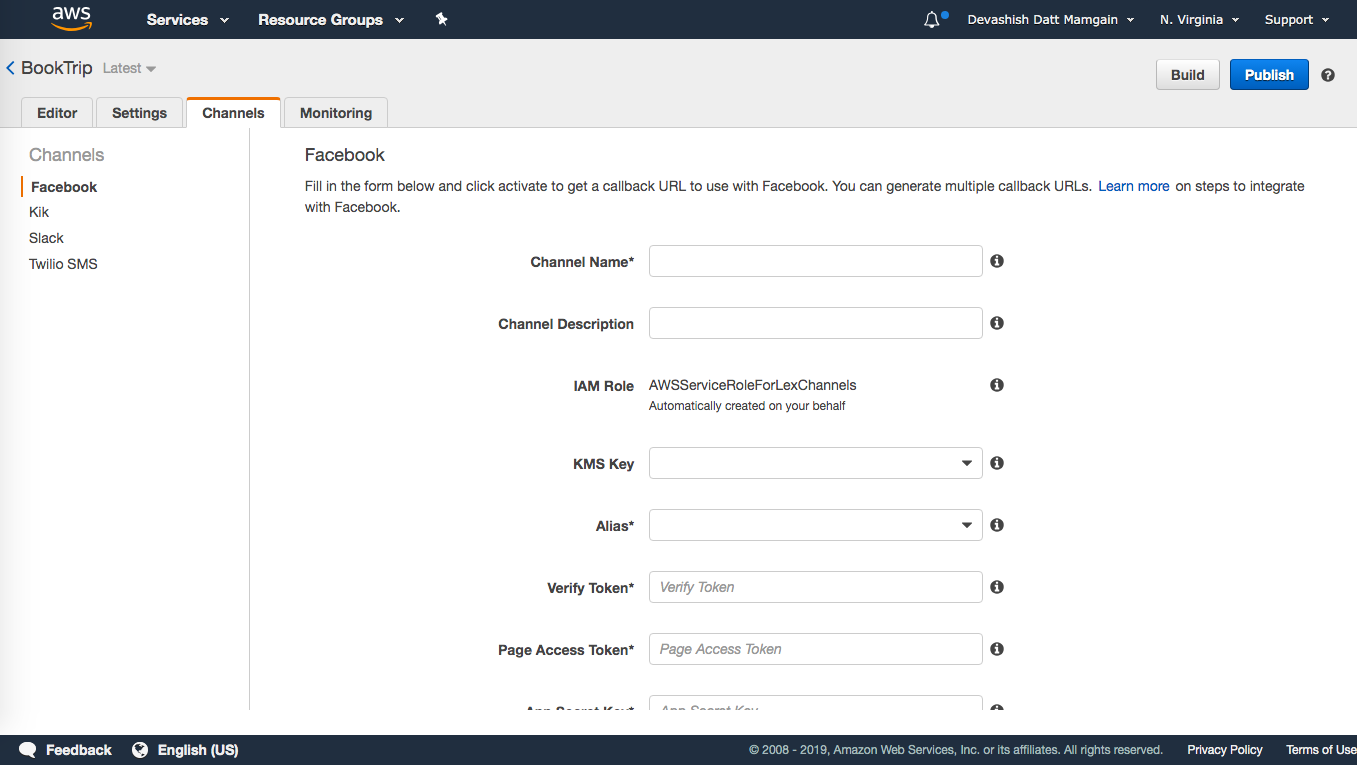
\includegraphics[width=0.6\linewidth]{chatbot58}

\tiny{(Ref : Dialogflow vs Lex vs Watson vs Wit vs Azure Bot | Which Chatbot Service Platform To Use?)}
\end{center}
\end{frame}

%%%%%%%%%%%%%%%%%%%%%%%%%%%%%%%%%%%%%%%%%%%%%%%%%%%%%%%%%%%
 \begin{frame}[fragile]\frametitle{IBM Watson Assistant}
\begin{itemize}
\item Has support for searching for an answer from the knowledge base 
\item First, you need to create a Skill and then go to Assistant to integrate it with other channels.
\end{itemize}

\begin{center}
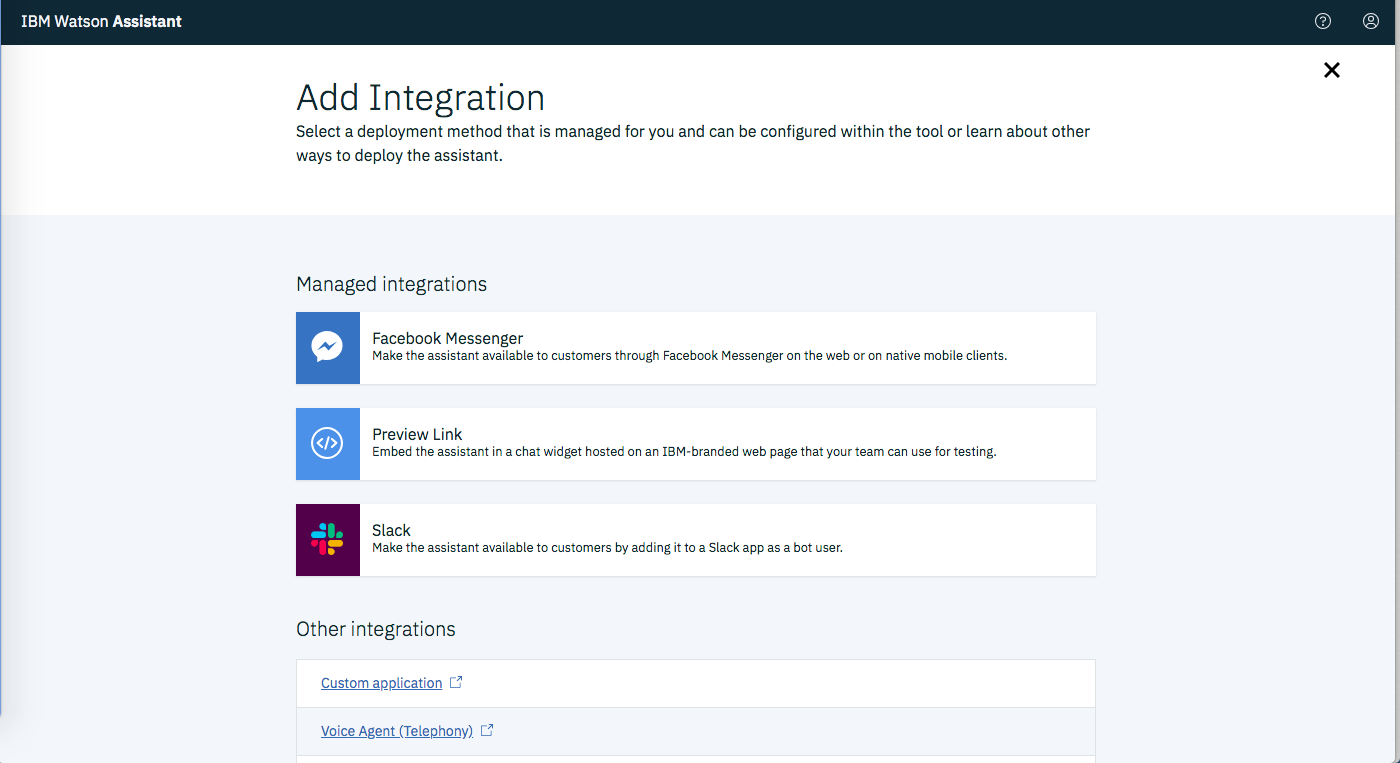
\includegraphics[width=0.6\linewidth]{chatbot59}

\tiny{(Ref : Dialogflow vs Lex vs Watson vs Wit vs Azure Bot | Which Chatbot Service Platform To Use?)}
\end{center}
\end{frame}

%%%%%%%%%%%%%%%%%%%%%%%%%%%%%%%%%%%%%%%%%%%%%%%%%%%%%%%%%%%
 \begin{frame}[fragile]\frametitle{Microsoft LUIS, Azure Bot Service}
\begin{itemize}
\item Web interface is available to create and publish bots which is fairly easy to understand.
\end{itemize}

\begin{center}
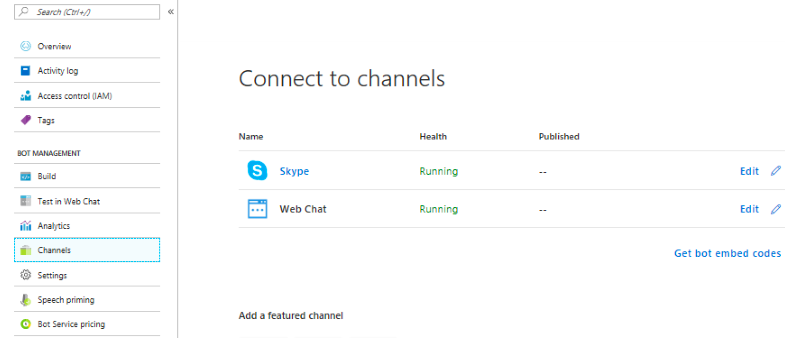
\includegraphics[width=0.6\linewidth]{chatbot60}

\tiny{(Ref : Dialogflow vs Lex vs Watson vs Wit vs Azure Bot | Which Chatbot Service Platform To Use?)}
\end{center}
\end{frame}


%%%%%%%%%%%%%%%%%%%%%%%%%%%%%%%%%%%%%%%%%%%%%%%%%%%%%%%%%%%
 \begin{frame}[fragile]\frametitle{Conversation Platforms}
We will be looking more closely at Rasa Platform\ldots
\end{frame}

%%%%%%%%%%%%%%%%%%%%%%%%%%%%%%%%%%%%%%%%%%%%%%%%%%%%%%%%%%%
\begin{frame}[fragile]\frametitle{Rasa Chatbot Architecture}


\begin{center}
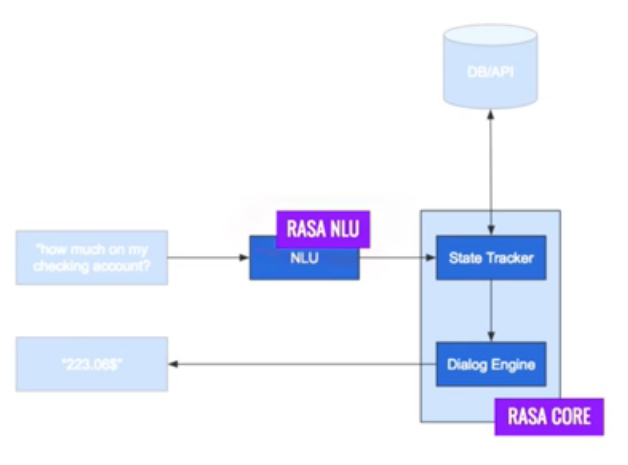
\includegraphics[width=0.6\linewidth]{rasa26}
\end{center}

Machine Learning based and in Python.

{\tiny (Ref: The talk would be about Rasa, an open-source chatbots platform - Nathan Zylbersztejn)}

\end{frame}



%%%%%%%%%%%%%%%%%%%%%%%%%%%%%%%%%%%%%%%%%%%%%%%%%%%%%%%%%%%%%%%%%%%%%%%%%%%%%%%%%%
\begin{frame}[fragile]\frametitle{}
\begin{center}
{\Large Why Rasa?}
\end{center}
\end{frame}

%%%%%%%%%%%%%%%%%%%%%%%%%%%%%%%%%%%%%%%%%%%%%%%%%%%%%%%%%%%
\begin{frame}[fragile]\frametitle{Rasa Stack Work-flow}


\begin{center}
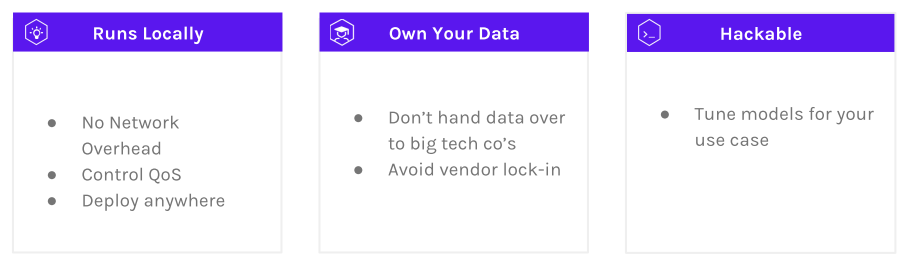
\includegraphics[width=\linewidth]{rasa14}
\end{center}


{\tiny (Ref: Conversational AI: Building clever chatbots - Tom Bocklisch)}

\end{frame}


%%%%%%%%%%%%%%%%%%%%%%%%%%%%%%%%%%%%%%%%%%%%%%%%%%%%%%%%%%%
 \begin{frame}[fragile]\frametitle{Advantages of Rasa}
\begin{itemize}
% \item Many chatbot platforms are currently available, from rudimentary rule-based AIML (Artificial Intelligence Markup Language), to highly sophisticated AI bots. 
\item Some popular chatbot platforms are API.ai, Wit.ai, Facebook APIs, Microsoft LUIS, IBM Watson, etc. are HOSTED services, meaning they send data over net.
\item RASA-NLU builds a local NLU (Natural Language Understanding) model for extracting intent and entities from a conversation. No data is passed over net.
\item It's open source, fully local and above all, free! 
\item It is also compatible with wit.ai, LUIS, or api.ai, so you can migrate your chat application data into the RASA-NLU model.
\end{itemize}
\end{frame}

%%%%%%%%%%%%%%%%%%%%%%%%%%%%%%%%%%%%%%%%%%%%%%%%%%%%%%%%%%%
 \begin{frame}[fragile]\frametitle{Why Local? - Security}
\begin{itemize}
\item Enterprises (and their customers) want AI assistants, not FAQ chatbots, but they're difficult to build; if you're not Google, and that is where Rasa comes in.
\item Fully controlling and owning your IP and data is crucial, and can't be done using cloud APIs. In the age of GDPR, HIPAA companies run Rasa on-premise or in a private cloud.
\end{itemize}

{\tiny (Ref: Our Open Source Community Is Growing Faster than Ever. Weren't Chatbots Meant to Be Dead? - Rasa Community Update - Alexander Weidauer )}
\end{frame}

%%%%%%%%%%%%%%%%%%%%%%%%%%%%%%%%%%%%%%%%%%%%%%%%%%%%%%%%%%%
 \begin{frame}[fragile]\frametitle{Control}
\begin{itemize}
\item You don't have to hand over your data to FB/MSFT/GOOG
\item You don't have to make a https call to parse every message.
\item You can tune models to work well on your particular use case.
\end{itemize}
\end{frame}


%%%%%%%%%%%%%%%%%%%%%%%%%%%%%%%%%%%%%%%%%%%%%%%%%%%%%%%%%%%
 \begin{frame}[fragile]\frametitle{State Machines}
Everyone uses state machines and state machines don't scale


\begin{center}
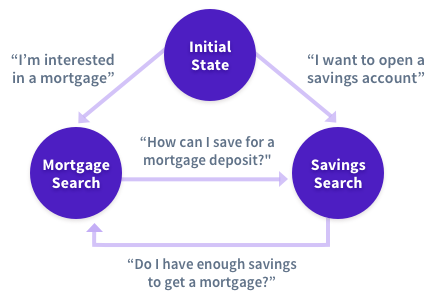
\includegraphics[width=0.6\linewidth,keepaspectratio]{chatbot22}

\end{center}

But then how to handle ``Straying from the happy path''?

{\tiny (Ref: A New Approach to Conversational Software - Alan Nichol)}
\end{frame}

%%%%%%%%%%%%%%%%%%%%%%%%%%%%%%%%%%%%%%%%%%%%%%%%%%%%%%%%%%%
 \begin{frame}[fragile]\frametitle{Rasa Approach}
 
 How can we use machine learning to move beyond the bag-of-rules approach?
 
\begin{itemize}
\item The Rasa Approach: flowcharts are useful for doing the initial design of a bot and describing a few of the happy paths, but you shouldn't take them literally and hard-code a bunch of rules. We've seen many times how this approach doesn't scale beyond simple conversations.
\item With Rasa Core, you manually specify all of the things your bot can say and do. We call these actions. One action might be to greet the user, another might be to call an API, or query a database. Then you train a probabilistic model to predict which action to take given the history of a conversation.
\end{itemize}

{\tiny (Ref: A New Approach to Conversational Software - Alan Nichol)}


\end{frame}

%%%%%%%%%%%%%%%%%%%%%%%%%%%%%%%%%%%%%%%%%%%%%%%%%%%%%%%%%%%
 \begin{frame}[fragile]\frametitle{Rasa Approach}
 
\begin{columns}
\begin{column}[T]{0.5\linewidth}

In interactive learning mode, you provide step-by-step feedback on what your bot decided to do. It's kind of like reinforcement learning, but with feedback on every single step (rather than just at the end of the conversation).

When your bot chooses the wrong action, you tell it what the right one would have been. The model updates itself immediately (so you are less likely to encounter the same mistake again) and once you finish, the conversation gets logged to a file and added to your training data.
\end{column}
\begin{column}[T]{0.5\linewidth}

\begin{center}
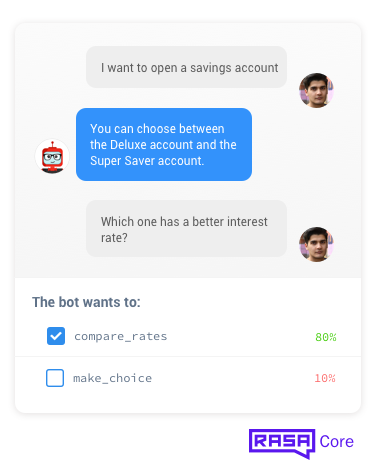
\includegraphics[width=\linewidth,keepaspectratio]{chatbot23}

\end{center}

{\tiny (Ref: A New Approach to Conversational Software - Alan Nichol)}

\end{column}
\end{columns}
\end{frame}

%%%%%%%%%%%%%%%%%%%%%%%%%%%%%%%%%%%%%%%%%%%%%%%%%%%%%%%%%%%
 \begin{frame}[fragile]\frametitle{Rasa Approach}
 

\begin{itemize}
\item You've instantly resolved an edge case, without staring at your code for ages figuring out what went wrong. And because you're providing step-by-step feedback, rather than a single reward at the end, you're teaching the system much more directly what's right and wrong.
\item  From experience it was found that, a couple of dozen short conversations are enough to get a first version of your system running.
\end{itemize}

{\tiny (Ref: A New Approach to Conversational Software - Alan Nichol)}


\end{frame}

%%%%%%%%%%%%%%%%%%%%%%%%%%%%%%%%%%%%%%%%%%%%%%%%%%%%%%%%%%%
 \begin{frame}[fragile]\frametitle{Other Reasons}

Rasa Stack is the leading open-source machine learning toolkit for developers to extend bots beyond answering simple questions.

Following figures are of Oct, 2018:

\begin{center}
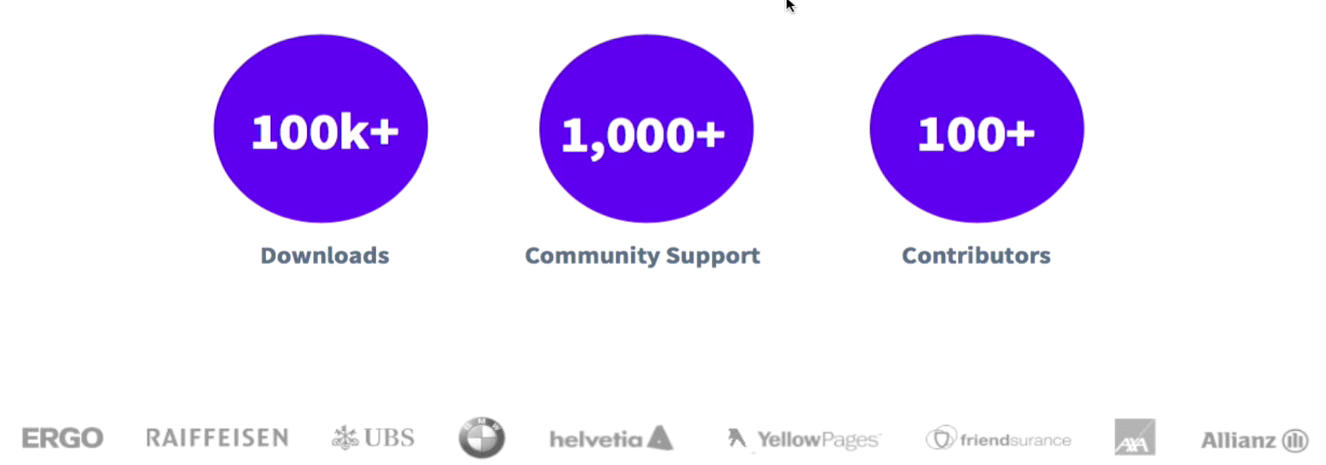
\includegraphics[width=\linewidth]{rasa19}
\end{center}


{\tiny (Ref: Building Conversational AI w Rasa Stack | Alan Nichol at PyBay2018)}

\end{frame}


%%%%%%%%%%%%%%%%%%%%%%%%%%%%%%%%%%%%%%%%%%%%%%%%%%%%%%%%%%%
 \begin{frame}[fragile]\frametitle{Can't we develop the chatbot ourselves?}

\begin{itemize}
\item Its not simple/mundane software development. Need people with varied backgrounds apart from developers, especially ML/DL/NLP.
\item Conversational AI (meaning, the one thats more than atomic Q and A) is a hard problem. Even the biggies haven't cracked it fully (Google's duplex can do only one or two things!!).
\item Softwrae patterns are not developed yet.
\item Rasa helps in taking us at some level and being open source you can help it grow further.
\end{itemize}


{\tiny (Ref: Building Conversational AI w Rasa Stack | Alan Nichol at PyBay2018)}

\end{frame}

%%%%%%%%%%%%%%%%%%%%%%%%%%%%%%%%%%%%%%%%%%%%%%%%%%%%%%%%%%%
 \begin{frame}[fragile]\frametitle{Is Rasa better than others?}
\begin{itemize}
\item Not too much, as for NLU capabilities, even compared to Google (Dialoglow), Facebook (Wit.API), etc, as per Benchmark study done by TU Munich
\item Depends very much on the training data.
\item But being open source and native, makes it a lot more attractive.
\item No data over Internet makes it fast and secure.
\item Sustainable: Not a fly-by-night operator. AT least you have full source that works!! (Apple acquired and closed init.ai)
\end{itemize}

{\tiny (Ref: The talk would be about Rasa, an open-source chatbots platform - Nathan Zylbersztejn)}

\end{frame}

%%%%%%%%%%%%%%%%%%%%%%%%%%%%%%%%%%%%%%%%%%%%%%%%%%%%%%%%%%%
 \begin{frame}[fragile]\frametitle{Btw, Rasa-X has arrived}
 What Rasa X is:
\begin{itemize}
\item Rasa X is a tool that helps you build, improve, and deploy AI Assistants that are powered by the Rasa framework. 
\item Rasa X runs on your own computer and you can deploy it to your own server. 
\item None of your conversations or training data are ever sent anywhere.
\item Rasa X comes in Community (\$0) and Enterprise (paid) editions. The community edition is free but not open source
\item Rasa X is a tool to learn from real conversations and improve your assistant.
\item Using it is totally optional. If you don’t want to, you can just use Rasa on its own.
\end{itemize}

 What Rasa X is NOT:
\begin{itemize}
\item It's not a hosted service.
\item It's not an all-in-one, point-and-click bot platform.
\end{itemize}
\end{frame}

%%%%%%%%%%%%%%%%%%%%%%%%%%%%%%%%%%%%%%%%%%%%%%%%%%%%%%%%%%%
 \begin{frame}[fragile]\frametitle{What happens to Rasa NLU and Rasa Core}
\begin{itemize}
\item Rasa NLU and Core (aka Rasa Stack) are now part of a single open source framework: Rasa, and version 1.0 is available
\item You can still use NLU and Core independently, they are just part of the same package now.
\item We will use Rasa NLU and Core in a traditional (old) way to understand how chatbot is developed
\end{itemize}
\end{frame}


